\documentclass[spanish,letterpaper,oneside]{article}

\def\documenttitle {El lugar perfecto}
\def\documentsubtitle {Temas selectos de matemáticas I · Cohorte SD26}
\def\documentsubject {Actividad 2 (Sesión 9) · Mediatrices, Bisectrices, Circuncentro e Incentro en GeoGebra}
\def\documentauthor {Mtro. Martín Jonathan de la Cruz Muñoz}
\def\coursename {Temas selectos de matemáticas I}
\def\coursecode {PFM02}

\def\universityname {Instituto de Investigación, Innovación y Estudios de Posgrado para la Educación del Estado de Nuevo León}
\def\universityfaculty {Maestría en Aprendizaje y Enseñanza de las Matemáticas}
\def\universitydepartment {Temas selectos de matemáticas I}
\def\universitydepartmentimage {img/iiiepe/marca-iiiepe.png}
\def\universitydepartmentimagecfg {height=1.75cm}
\def\universitylocation {Monterrey, Nuevo León}
\def\studentfullname {Mtro. Martín Jonathan de la Cruz Muñoz}
\def\studentid {00874}
\def\studentemail {martin.delacruz@campus.iiiepe.edu.mx}
\def\programperiod {2do periodo, agosto--noviembre de 2026 (SD26)}
\def\programmodality {Modalidad presencial y en línea}
\def\programshort {MAEM}

\def\authortable {
  \begin{tabular}{ll}
    \textbf{Alumno:} & \studentfullname \\
    Matrícula: & \studentid \\
    Correo institucional: & \studentemail \\
    Unidad: & \coursename \\
    Programa: & \programshort \\
    Periodo: & \programperiod \\
    & \\
    \multicolumn{2}{l}{Fecha de realización: 17 de octubre de 2026} \\
    \multicolumn{2}{l}{\universitylocation}
  \end{tabular}
}

\input{template}

\usepackage{helvet}
\renewcommand{\familydefault}{\sfdefault}
\usepackage{amsmath,amssymb,booktabs,array,longtable,pdflscape,tikz,tabularx,colortbl,pgfplots,enumitem,needspace}
\usepackage[most]{tcolorbox}
\usetikzlibrary{arrows.meta,positioning,calc,fit,backgrounds,babel}
\pgfplotsset{compat=1.18}

\definecolor{iiiepeNavy}{HTML}{163B5C}
\definecolor{iiiepeBlue}{HTML}{1F6F9F}
\definecolor{iiiepeAqua}{HTML}{20B7A8}
\definecolor{iiiepeOrange}{HTML}{F28C28}
\definecolor{iiiepePaper}{HTML}{F6F8F7}
\definecolor{iiiepeInk}{HTML}{1E2A32}
\definecolor{iiiepePale}{HTML}{EEF5F8}
\def\portraittitlecolor {iiiepeNavy}
\setcitestyle{authoryear,open={(},close={)}}

\newcommand{\insertcoverwatermark}{%
  \AddToShipoutPictureBG*{%
    \begin{tikzpicture}[remember picture,overlay]
      \node[opacity=.06,inner sep=0pt] at (current page.center)
      {
\includegraphics[width=.58\paperwidth]{img/iiiepe/logo-puntos.png}};
    \end{tikzpicture}%
  }%
}

\newtcolorbox{propuestabox}[1][]{%
  enhanced,breakable,
  colback=iiiepePaper,colframe=iiiepeAqua!80!iiiepeNavy,
  boxrule=1pt,leftrule=4pt,arc=2pt,
  left=8pt,right=8pt,top=6pt,bottom=6pt,
  before skip=6pt,after skip=10pt,
  fonttitle=\bfseries\color{white},coltitle=white,
  colbacktitle=iiiepeNavy,
  attach boxed title to top left={xshift=8pt,yshift=-2pt},
  boxed title style={colback=iiiepeNavy,colframe=iiiepeNavy,arc=1pt},
  title={Propuesta didáctica},#1}

\setlength{\parskip}{5pt}\setlength{\parindent}{0pt}
\begin{document}\insertcoverwatermark\templatePortrait\templatePagecfg\templateFinalcfg\fancyfoot{}\fancyfoot[L]{\scriptsize IIIEPE · MAEM · SD26}\fancyfoot[C]{\scriptsize\thepage}\fancyfoot[R]{\scriptsize Actividad 2}\setstretch{1.25}\raggedbottom

\section{Retos presenciales de equidistancia (regla y compás)}
La Sesión 9 del Bloque II aborda los lugares geométricos de equidistancia a partir de tres situaciones escolares contextualizadas \citep{iiiepe2026_s9,sep2024_fase6}:
\begin{enumerate}
  \item \textbf{Reto 1 (¿Dónde colocarías el bebedero?):} Colocar un bebedero equidistante de dos salones puntuales $A$ y $B$. Al buscar un segundo punto y comprobar distancias, el alumnado descubre que existen \textbf{infinitos puntos posibles}, caracterizados por la doble implicación $\overline{PA}=\overline{PB} \iff P \in m_{AB}$, donde $m_{AB}$ es la \textbf{mediatriz} del segmento $\overline{AB}$ \citep{euclides_elementos}. La suficiencia sigue por criterio LAL ($\triangle PMA \cong \triangle PMB$) y la necesidad por criterio LLL ($PA=PB$, $MA=MB$, $PM$ común $\implies \angle PMA = \angle PMB = 90^\circ$). \textit{Posibles dudas atendidas:} superar la creencia de que solo el punto medio $M$ funciona, elegir abertura del compás $> AB/2$ y medir distancia directa al punto.
  \item \textbf{Reto 2 (¿Habrá otro lugar posible entre dos caminos?):} Ubicar un árbol equidistante de dos caminos rectilíneos concurrentes (Camino 1 y Camino 2). Con compás se trazan arcos desde puntos simétricos sobre ambos lados y se determina la \textbf{bisectriz interior} del ángulo formado: dado que la distancia de un punto a una recta se mide perpendicularmente, todo punto $P$ sobre ella satisface $\triangle OHP \cong \triangle OKP$ (criterio AAL/hipotenusa-ángulo) e iguala las distancias perpendiculares ($PH = PK$). Además, conviene distinguir que la bisectriz del ángulo suplementario exterior también cumple equidistancia respecto a las rectas prolongadas y resulta perpendicular a la bisectriz interior.
  \item \textbf{Reto 3 (Equidistancia a tres salones $A$, $B$ y $C$):} Al unir los tres salones no colineales formando $\triangle ABC$, basta construir las mediatrices de dos lados (por ejemplo $\overline{BC}$ y $\overline{AC}$). Si $O$ pertenece a ambas, cumple $OB = OC$ y $OA = OC$; por tanto, por transitividad $OA = OB$, garantizando que $O$ pertenece también a la tercera mediatriz. Este punto único de concurrencia es el \textbf{circuncentro ($O$)}, centro de la circunferencia circunscrita a $\triangle ABC$. \textit{Posibles dudas atendidas:} verificar que dos mediatrices bastan (la tercera es comprobación), distinguir el caso colineal degenerado (mediatrices paralelas sin solución) y el caso obtusángulo ($O$ exterior).
\end{enumerate}

\begin{figure}[htbp]
\centering
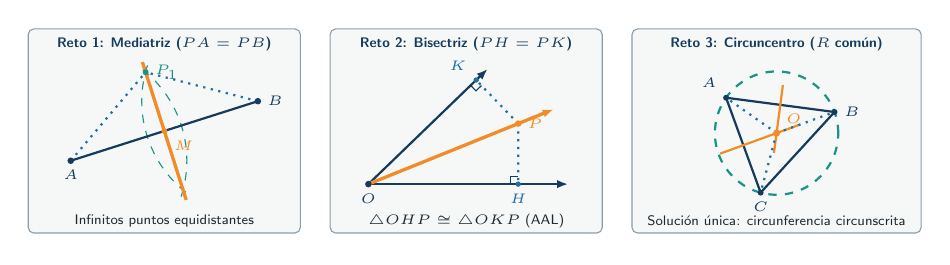
\begin{tikzpicture}[scale=0.54,font=\tiny]
  % Panel 1: Mediatriz (Reto 1)
  \begin{scope}[xshift=0cm]
    \draw[fill=iiiepePaper,draw=iiiepeNavy!50,rounded corners=2pt] (-0.2,-0.5) rectangle (6.2,4.3);
    \node[font=\tiny\bfseries,iiiepeNavy] at (3.0,3.95) {Reto 1: Mediatriz ($PA=PB$)};
    \coordinate (A1) at (0.8,1.2);
    \coordinate (B1) at (5.2,2.6);
    \coordinate (M1) at ($(A1)!0.5!(B1)$);
    \coordinate (P1a) at ($(M1)+1.45*(-0.303,0.953)$);
    \draw[iiiepeAqua!80!black,dashed] (A1) ++(-18:2.73) arc (-18:55:2.73);
    \draw[iiiepeAqua!80!black,dashed] (B1) ++(162:2.73) arc (162:235:2.73);
    \draw[iiiepeNavy,thick] (A1) -- (B1);
    \draw[iiiepeOrange,very thick] ($(M1)-1.70*(-0.303,0.953)$) -- ($(M1)+1.70*(-0.303,0.953)$);
    \draw[iiiepeBlue,dotted,thick] (A1) -- (P1a) (B1) -- (P1a);
    \fill[iiiepeNavy] (A1) circle (2.2pt) node[below] {$A$};
    \fill[iiiepeNavy] (B1) circle (2.2pt) node[right] {$B$};
    \fill[iiiepeOrange] (M1) circle (2pt) node[below right] {$M$};
    \fill[iiiepeAqua!80!black] (P1a) circle (2pt) node[right] {$P_1$};
    \node[iiiepeInk] at (3.0,-0.22) {Infinitos puntos equidistantes};
  \end{scope}

  % Panel 2: Bisectriz (Reto 2)
  \begin{scope}[xshift=7.1cm]
    \draw[fill=iiiepePaper,draw=iiiepeNavy!50,rounded corners=2pt] (-0.2,-0.5) rectangle (6.2,4.3);
    \node[font=\tiny\bfseries,iiiepeNavy] at (3.0,3.95) {Reto 2: Bisectriz ($PH=PK$)};
    \coordinate (O2) at (0.7,0.65);
    \coordinate (P2t) at ($(O2)+(22:3.8)$);
    \coordinate (H2) at ($(O2)+(0:{3.8*cos(22)})$);
    \coordinate (K2) at ($(O2)+(44:{3.8*cos(22)})$);
    \draw[-{Latex[length=1.4mm]},iiiepeNavy,thick] (O2) -- ++(0:4.7);
    \draw[-{Latex[length=1.4mm]},iiiepeNavy,thick] (O2) -- ++(44:3.9);
    \draw[-{Latex[length=1.4mm]},iiiepeOrange,very thick] (O2) -- ++(22:4.7);
    \draw[iiiepeBlue,dotted,thick] (P2t) -- (H2) (P2t) -- (K2);
    \draw[iiiepeNavy] (H2) ++(-0.18,0) -- ++(0,0.18) -- ++(0.18,0);
    \draw[iiiepeNavy] (K2) ++(224:0.18) -- ++(-46:0.18) -- ++(44:0.18);
    \fill[iiiepeNavy] (O2) circle (2.2pt) node[below] {$O$};
    \fill[iiiepeOrange] (P2t) circle (2.2pt) node[right] {$P$};
    \fill[iiiepeBlue] (H2) circle (1.8pt) node[below] {$H$};
    \fill[iiiepeBlue] (K2) circle (1.8pt) node[above left] {$K$};
    \node[iiiepeInk] at (3.0,-0.22) {$\triangle OHP\cong\triangle OKP$ (AAL)};
  \end{scope}

  % Panel 3: Circuncentro (Reto 3)
  \begin{scope}[xshift=14.2cm]
    \draw[fill=iiiepePaper,draw=iiiepeNavy!50,rounded corners=2pt] (-0.2,-0.5) rectangle (6.6,4.3);
    \node[font=\tiny\bfseries,iiiepeNavy] at (3.2,3.95) {Reto 3: Circuncentro ($R$ común)};
    \coordinate (O3) at (3.2,1.85);
    \coordinate (A3) at ($(O3)+(145:1.45)$);
    \coordinate (B3) at ($(O3)+(20:1.45)$);
    \coordinate (C3) at ($(O3)+(-105:1.45)$);
    \draw[iiiepeAqua!80!black,dashed,thick] (O3) circle (1.45);
    \draw[iiiepeNavy,thick] (A3) -- (B3) -- (C3) -- cycle;
    \draw[iiiepeOrange,thick] ($(O3)!-0.7!($(A3)!0.5!(B3)$)$) -- ($($(A3)!0.5!(B3)$)!-0.7!(O3)$);
    \draw[iiiepeOrange,thick] ($(O3)!-0.7!($(A3)!0.5!(C3)$)$) -- ($($(A3)!0.5!(C3)$)!-0.7!(O3)$);
    \draw[iiiepeBlue,dotted,thick] (O3) -- (A3) (O3) -- (B3) (O3) -- (C3);
    \fill[iiiepeNavy] (A3) circle (2pt) node[above left] {$A$};
    \fill[iiiepeNavy] (B3) circle (2pt) node[right] {$B$};
    \fill[iiiepeNavy] (C3) circle (2pt) node[below] {$C$};
    \fill[iiiepeOrange] (O3) circle (2.4pt) node[above right] {$O$};
    \node[iiiepeInk] at (3.2,-0.22) {Solución única: circunferencia circunscrita};
  \end{scope}
\end{tikzpicture}
\caption{Esquemas geométricos de validación para los tres retos presenciales de la Sesión 9 (mediatriz, bisectriz y circuncentro).}
\end{figure}

\section{Guía de trabajo ejecutada en GeoGebra Classic}

\subsection{Actividad a. Punto equidistante de tres vértices (Circuncentro $O$)}
Se construyó en GeoGebra Classic el triángulo escaleno acutángulo con vértices $A=(1,6)$, $B=(-3,-2)$ y $C=(6,1)$, sus tres mediatrices ($m_a, m_b, m_c$), el punto de intersección $O=(1,1)$ y los segmentos $OA, OB, OC$. Las mediciones certifican exactamente $OA = OB = OC = 5.00\text{ u}$ (radio de la circunferencia circunscrita).

\begin{figure}[htbp]
\centering
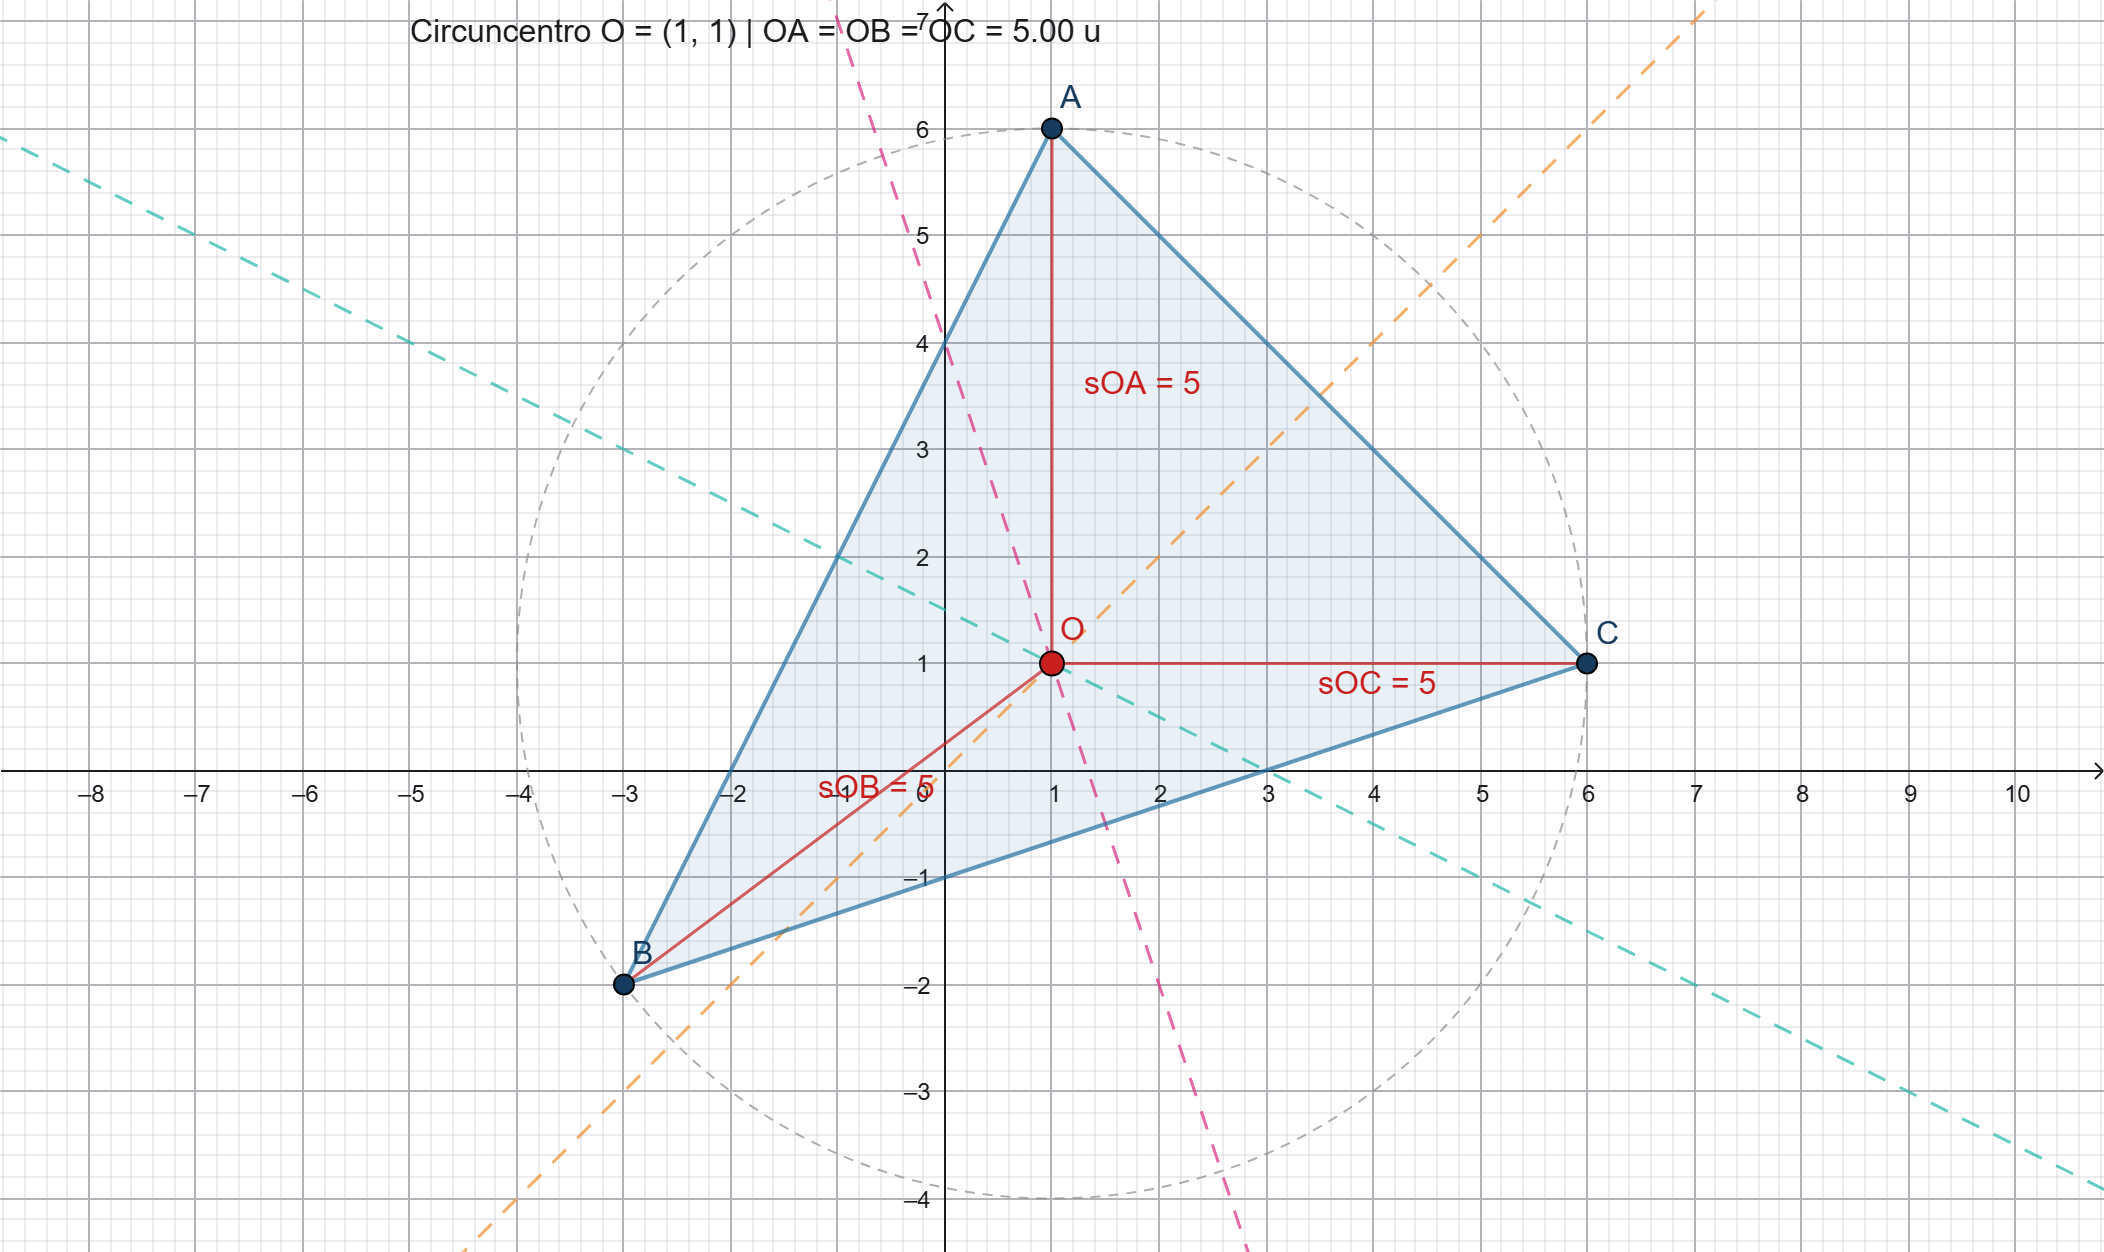
\includegraphics[width=0.84\linewidth]{img/geogebra/act2_a_mediatrices_equidistancia.png}
\caption{Actividad a (GeoGebra): Mediatrices, circuncentro $O=(1,1)$ y comprobación métrica $OA=OB=OC=5\text{ u}$.}
\end{figure}

\textbf{Respuestas a las preguntas de reflexión (Actividad a):} Las distancias $OA$, $OB$ y $OC$ son \textbf{iguales} ($5.00\text{ u}$ en la construcción). En consecuencia, el punto $O$ tiene la característica fundamental de \textbf{equidistar de los tres vértices del triángulo}, lo que permite trazar una circunferencia con centro en $O$ que pasa exactamente por $A$, $B$ y $C$.

\subsection{Actividad b. Ubicación de $O$ según el tipo de triángulo}
Se manipuló el triángulo en GeoGebra para inspeccionar los tres casos angulares:
\begin{itemize}
  \item \textbf{Triángulo acutángulo} ($A=(1,6), B=(-3,-2), C=(6,1)$): el circuncentro $O$ queda \textbf{en el interior} del triángulo.
  \item \textbf{Triángulo rectángulo} ($A=(-3,4), B=(-3,-2), C=(5,-2)$, ángulo recto en $B=90^\circ$): el circuncentro $O=(1,1)$ queda \textbf{sobre el punto medio de la hipotenusa $\overline{AC}$} (consecuencia directa del Teorema de Tales).
  \item \textbf{Triángulo obtusángulo} ($A=(-4,0), B=(5,0), C=(0,-1.5)$): el circuncentro $O$ queda \textbf{en el exterior} del triángulo, frente al ángulo obtuso.
\end{itemize}

\begin{figure}[htbp]
\centering
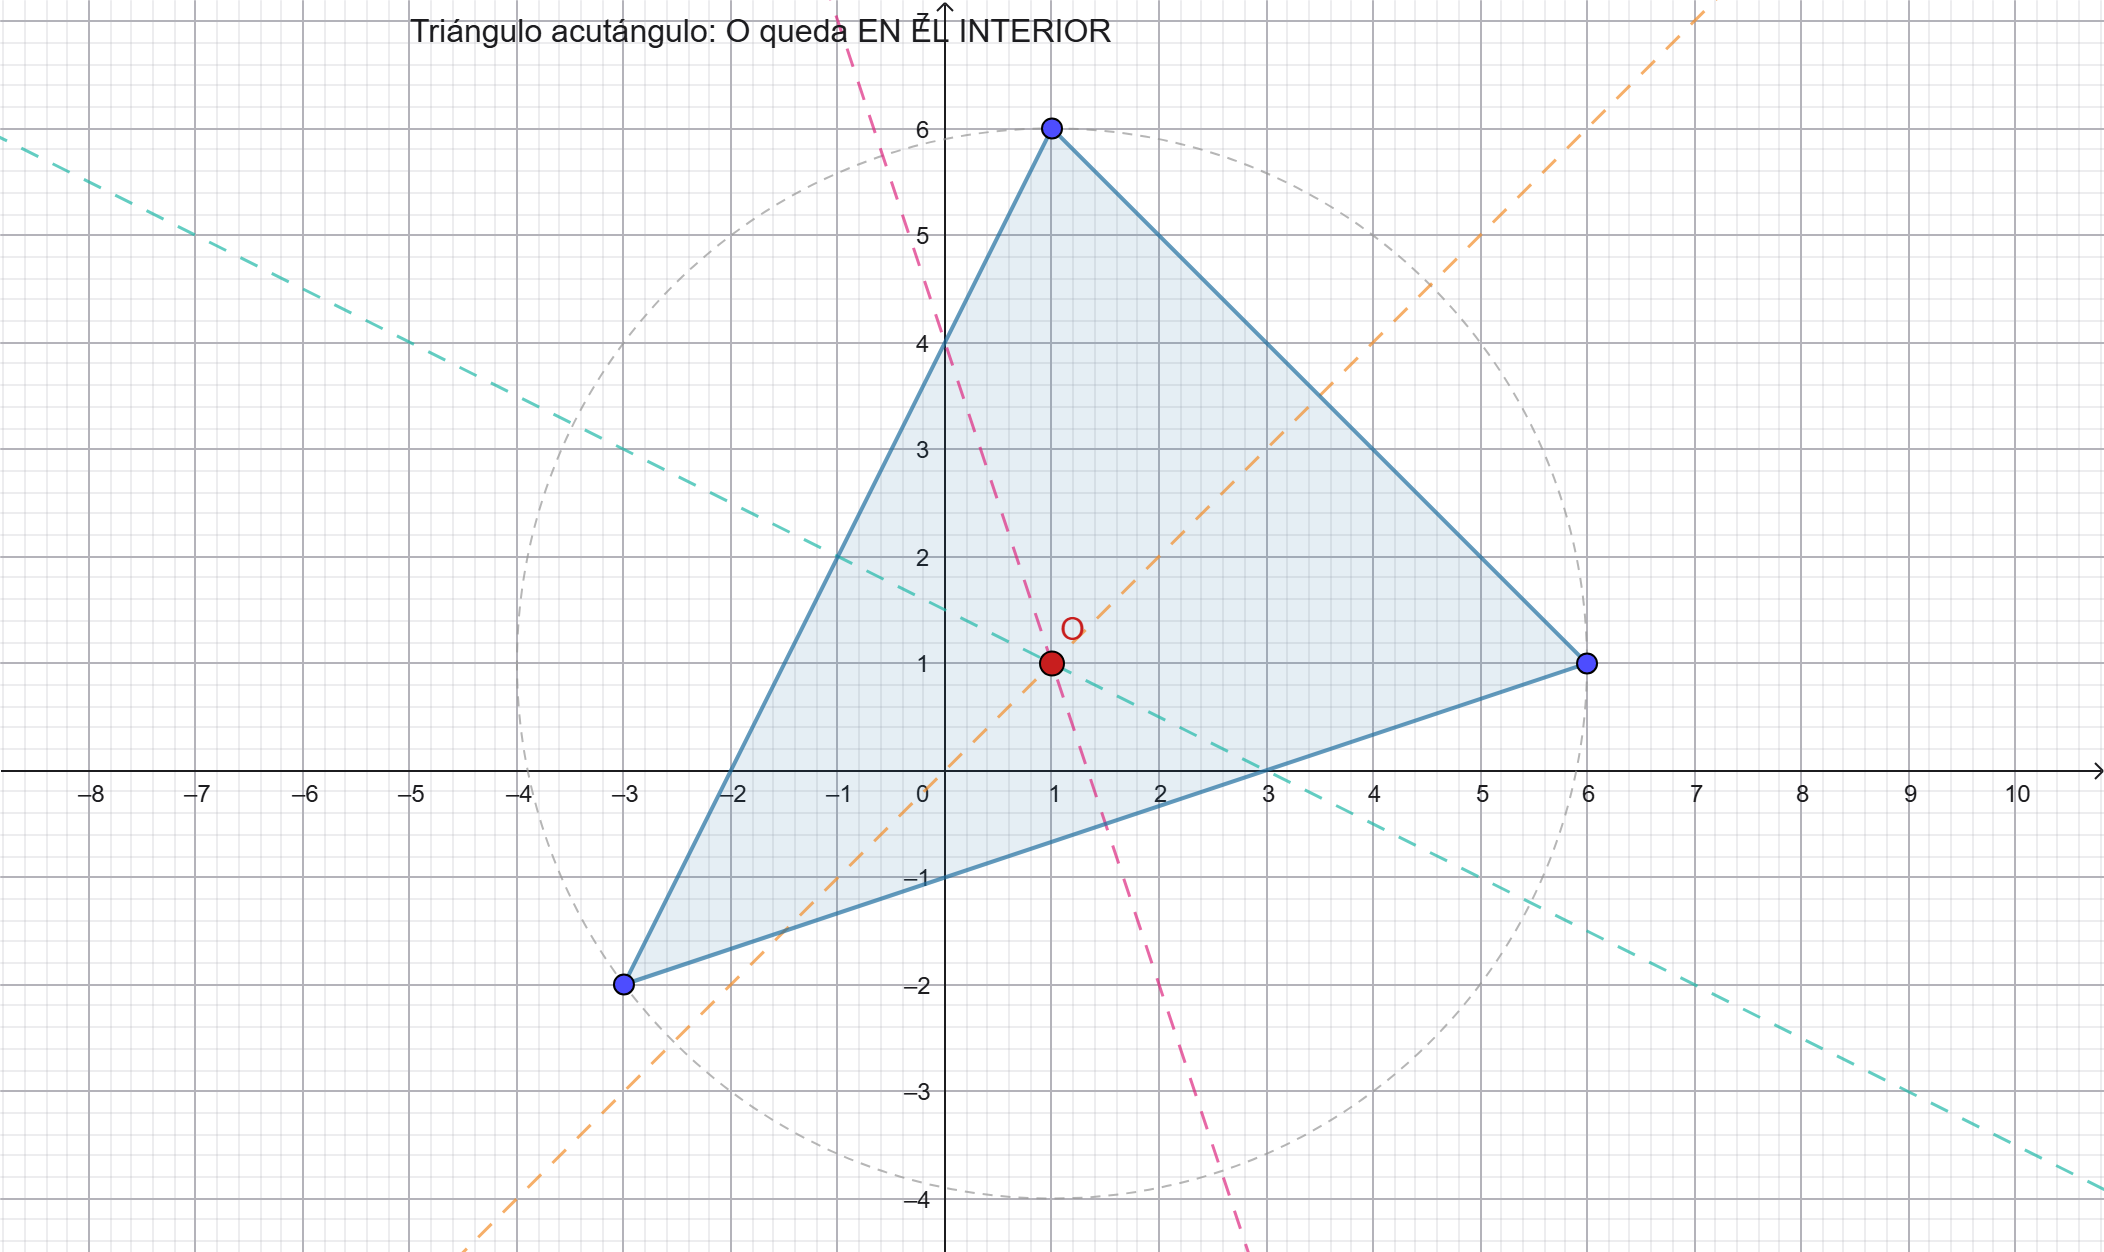
\includegraphics[width=0.32\linewidth]{img/geogebra/act2_b1_circuncentro_acutangulo.png}\hfill
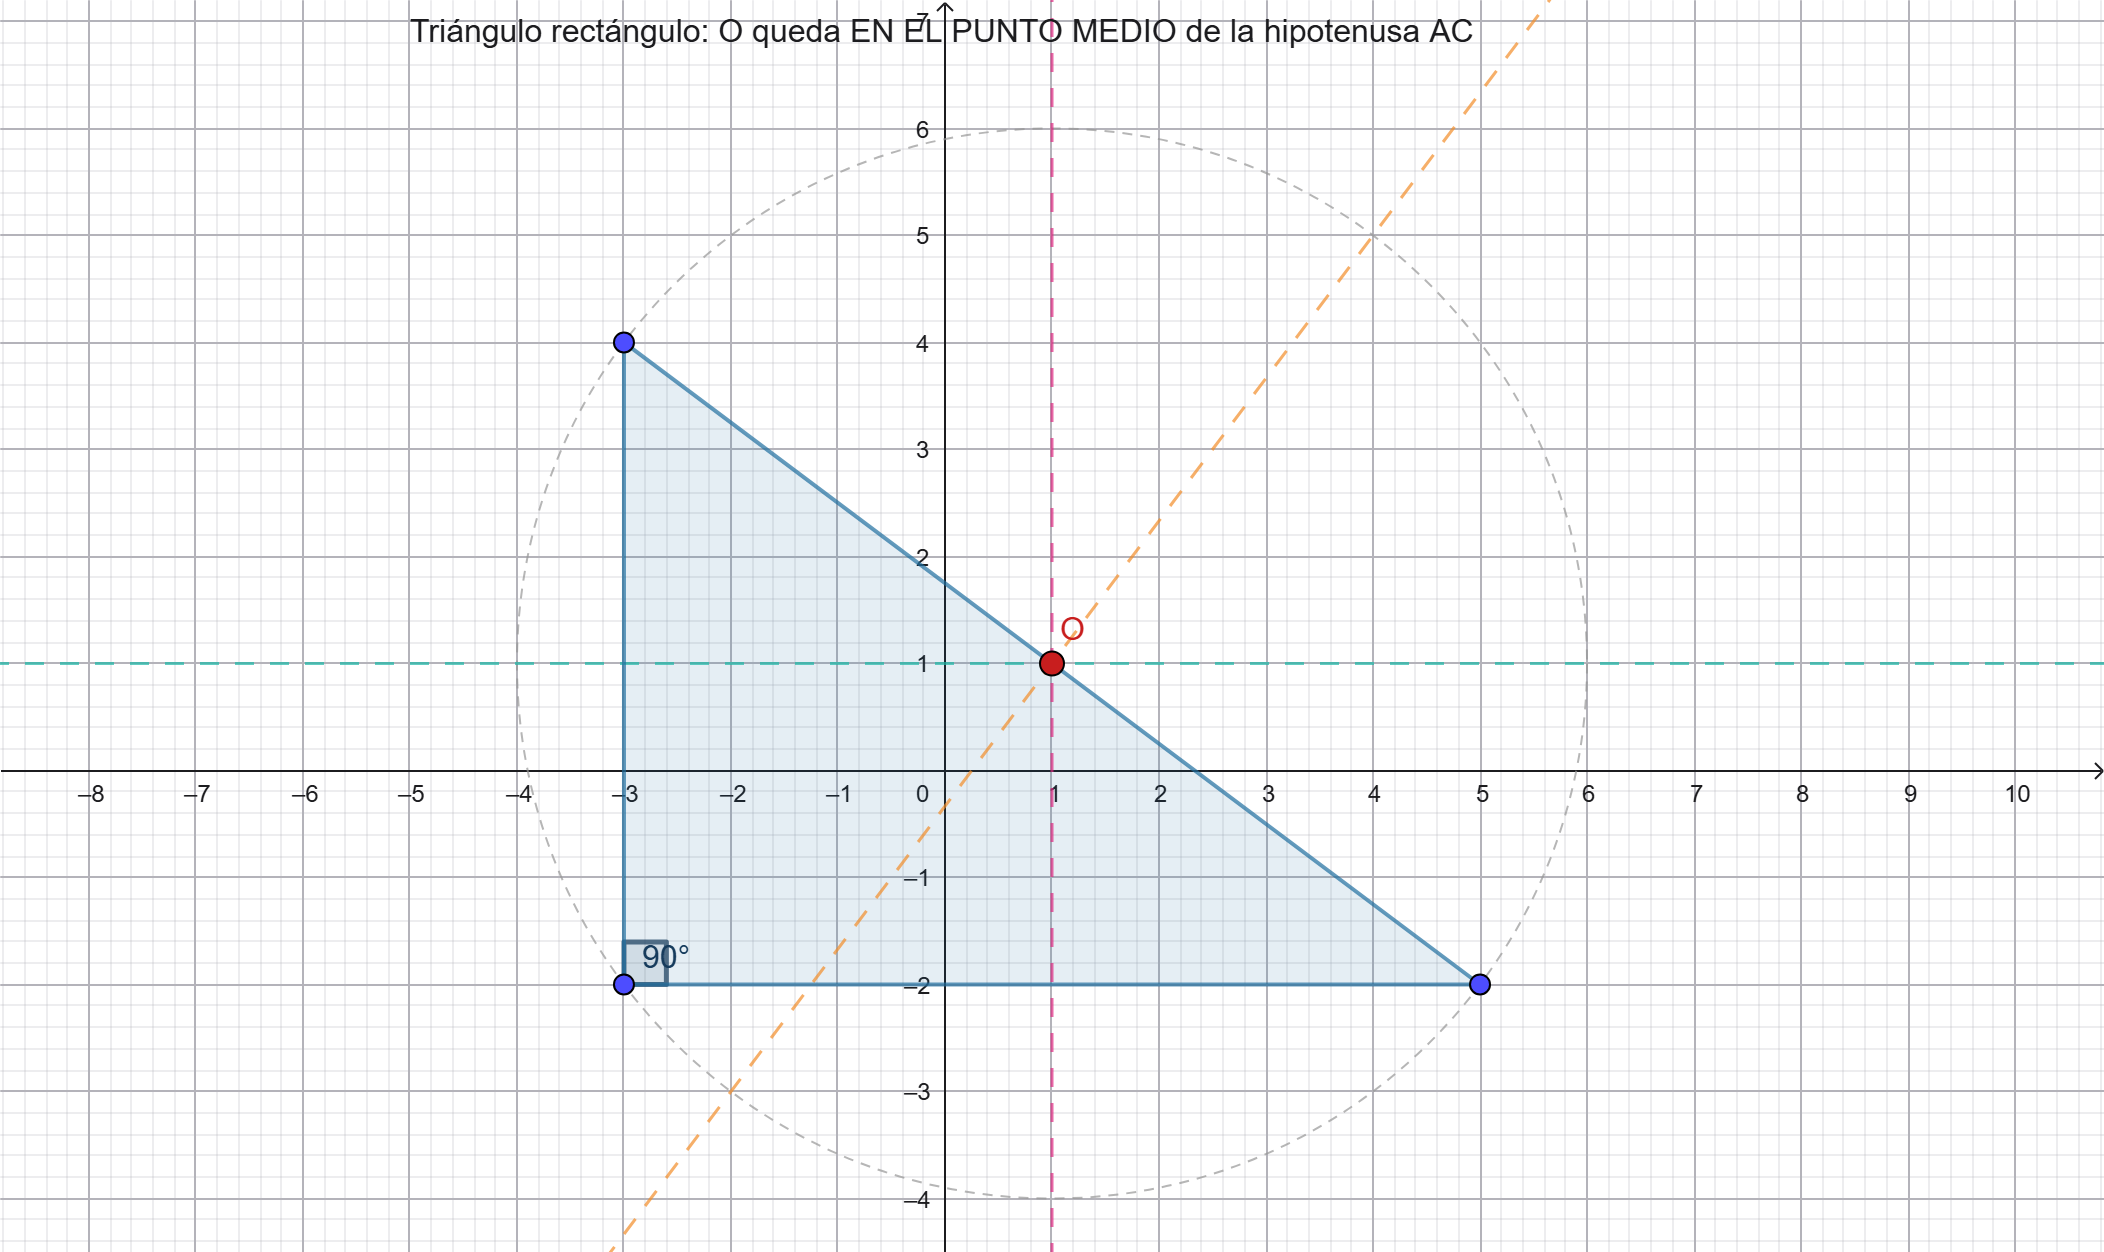
\includegraphics[width=0.32\linewidth]{img/geogebra/act2_b2_circuncentro_rectangulo.png}\hfill
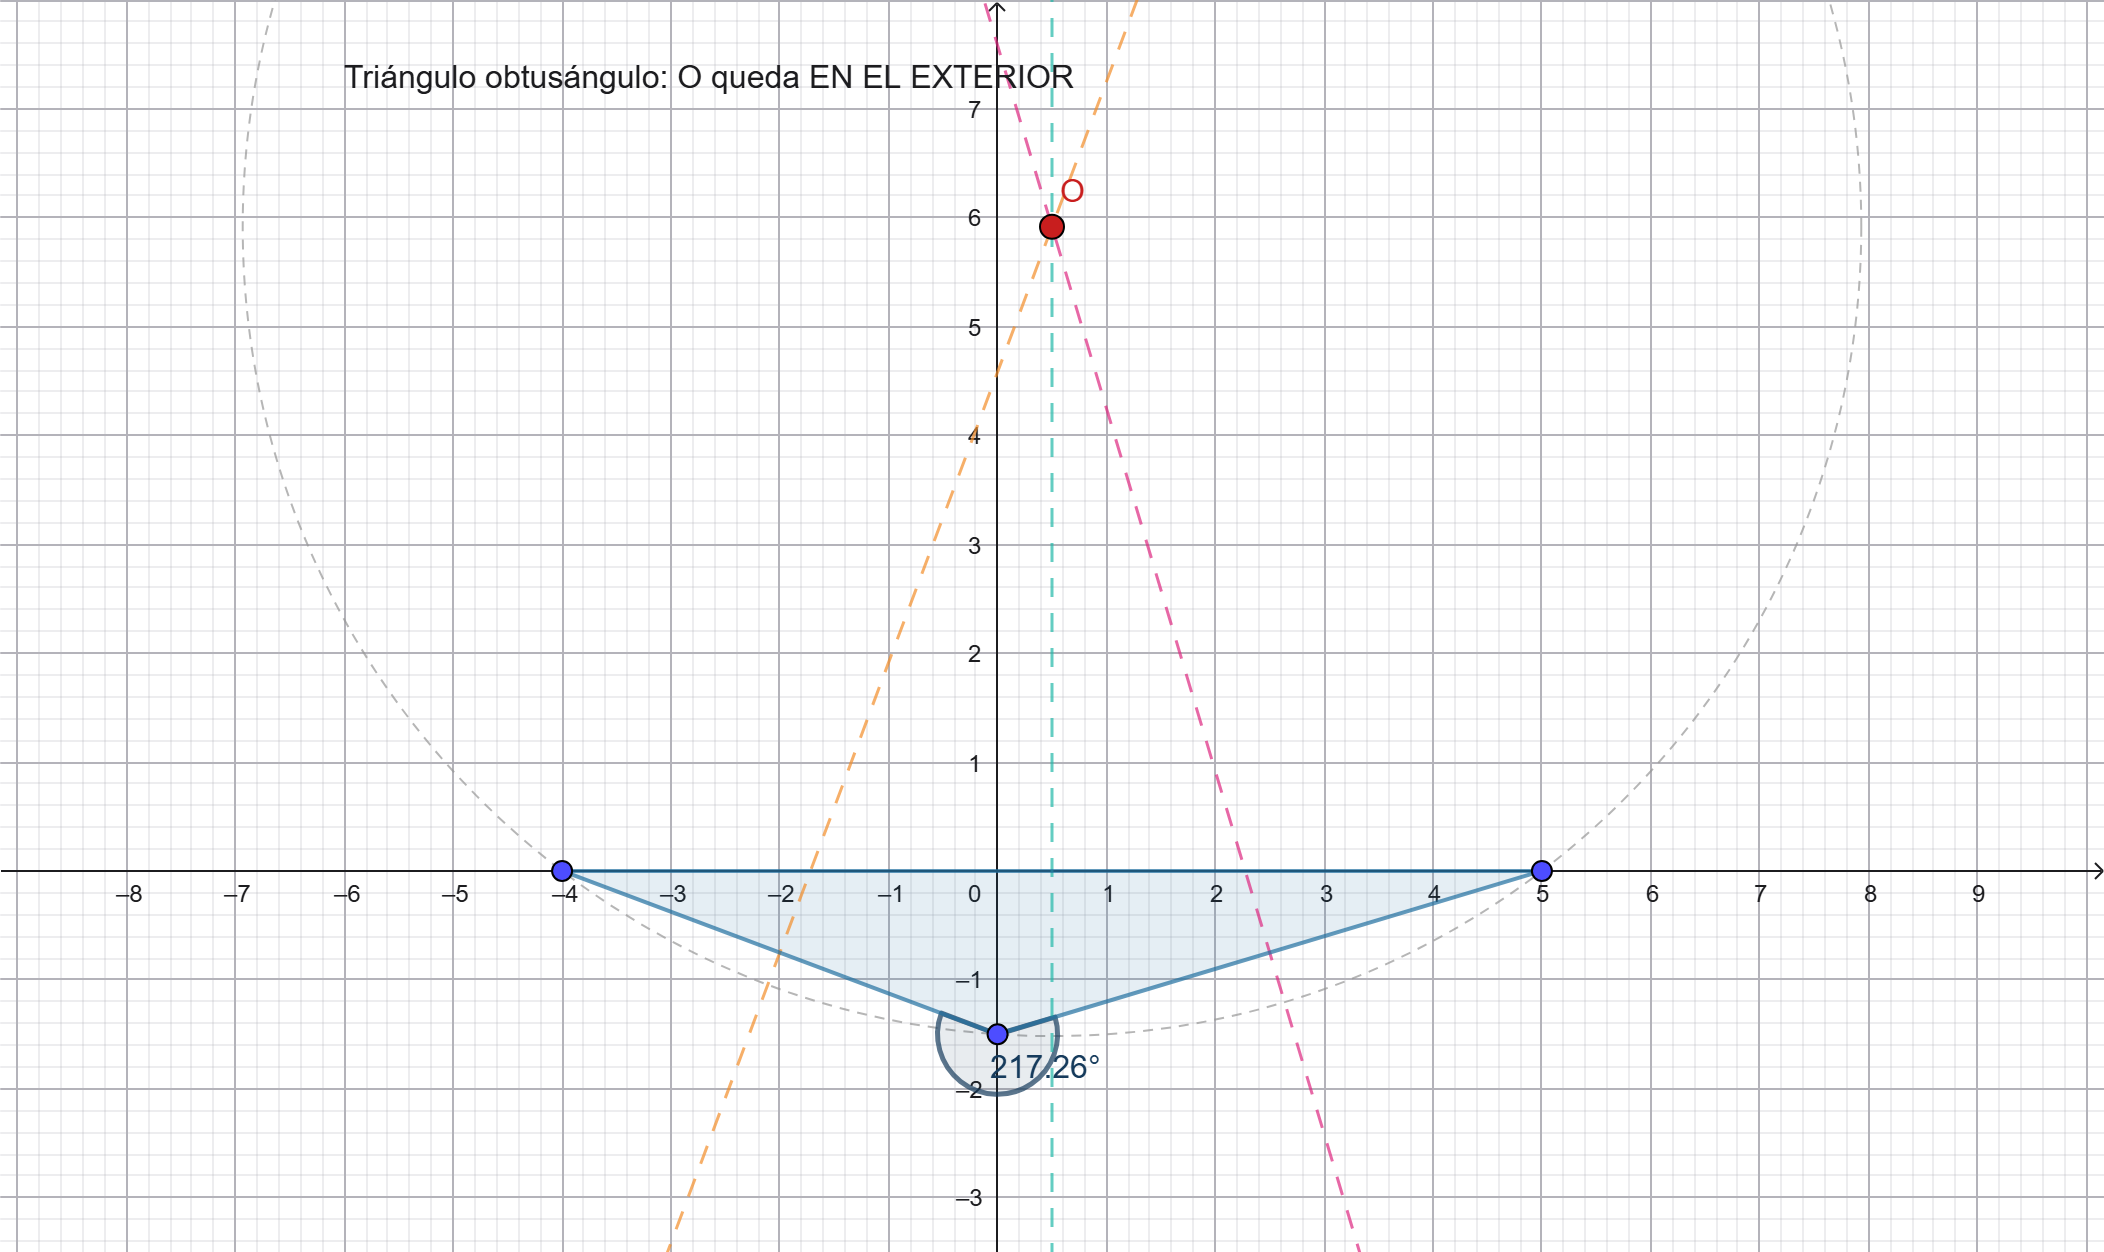
\includegraphics[width=0.32\linewidth]{img/geogebra/act2_b3_circuncentro_obtusangulo.png}
\caption{Actividad b (GeoGebra): Posición del circuncentro $O$ en triángulo acutángulo (interior), rectángulo (punto medio de la hipotenusa) y obtusángulo (exterior).}
\end{figure}

\textbf{Respuesta a la pregunta de reflexión (Actividad b):} La ubicación de $O$ depende del mayor ángulo interior del triángulo: si los tres ángulos son agudos, $O$ permanece en el interior; cuando un ángulo alcanza $90^\circ$, las mediatrices de los catetos cortan exactamente en el punto medio de la hipotenusa; si un ángulo supera $90^\circ$, las mediatrices convergen fuera del triángulo. En contextos escolares reales (como ubicar un bebedero), un circuncentro exterior advertiría que el punto óptimo geométrico queda fuera del patio triangular delimitado.

\subsection{Actividad c. Exploración de bisectrices interiores e Incentro $I$}
Ocultando las mediatrices y trazando las tres bisectrices interiores ($b_A, b_B, b_C$), se identificó su punto de concurrencia $I$ (\textbf{incentro}) junto con la circunferencia inscrita tangente a los tres lados en los tres tipos de triángulos.

\begin{figure}[htbp]
\centering
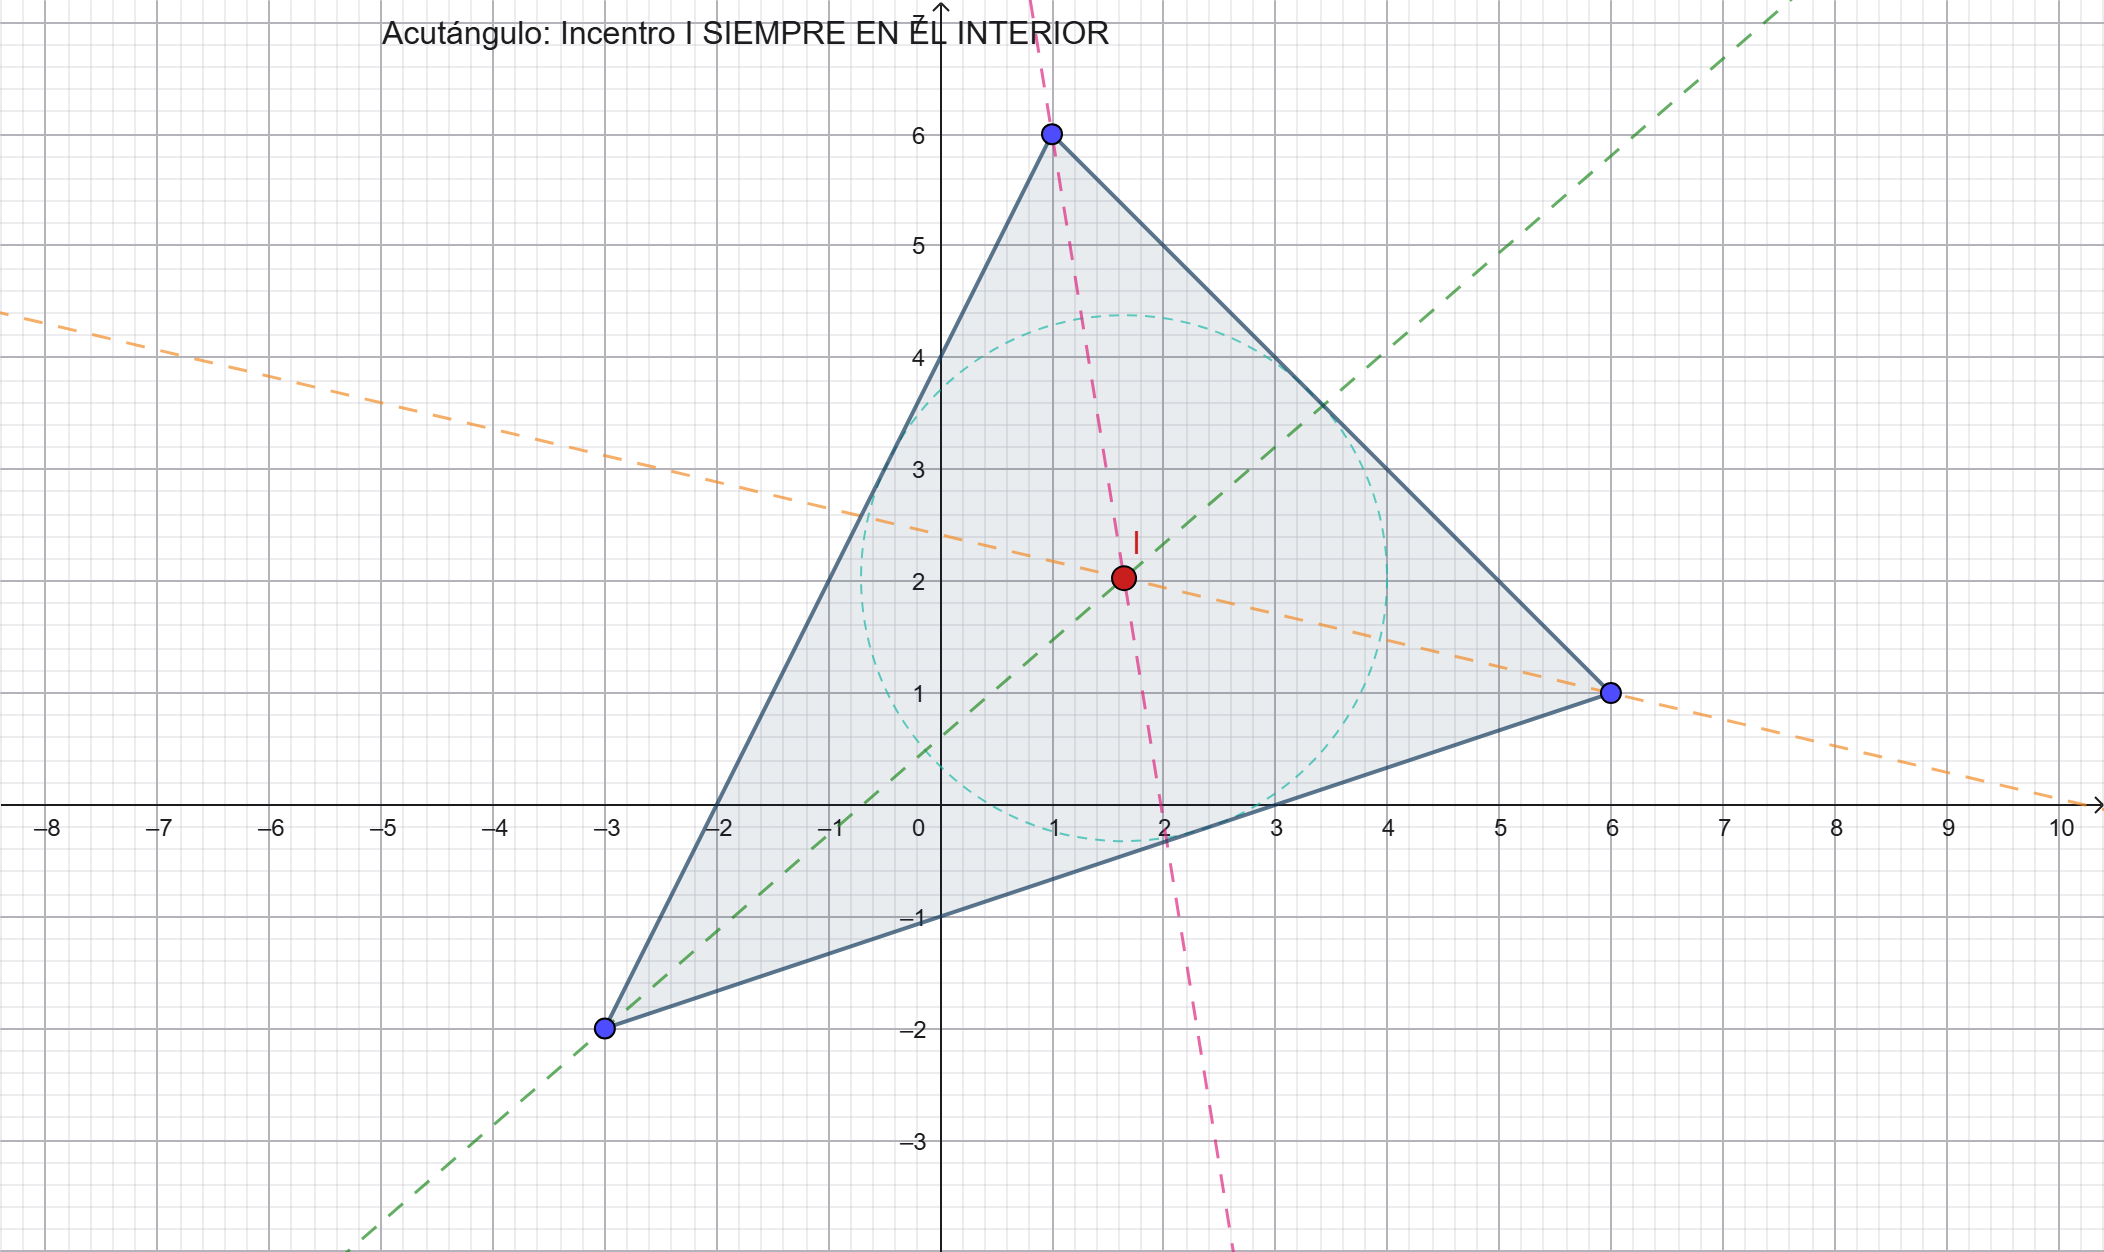
\includegraphics[width=0.32\linewidth]{img/geogebra/act2_c1_incentro_acutangulo.png}\hfill
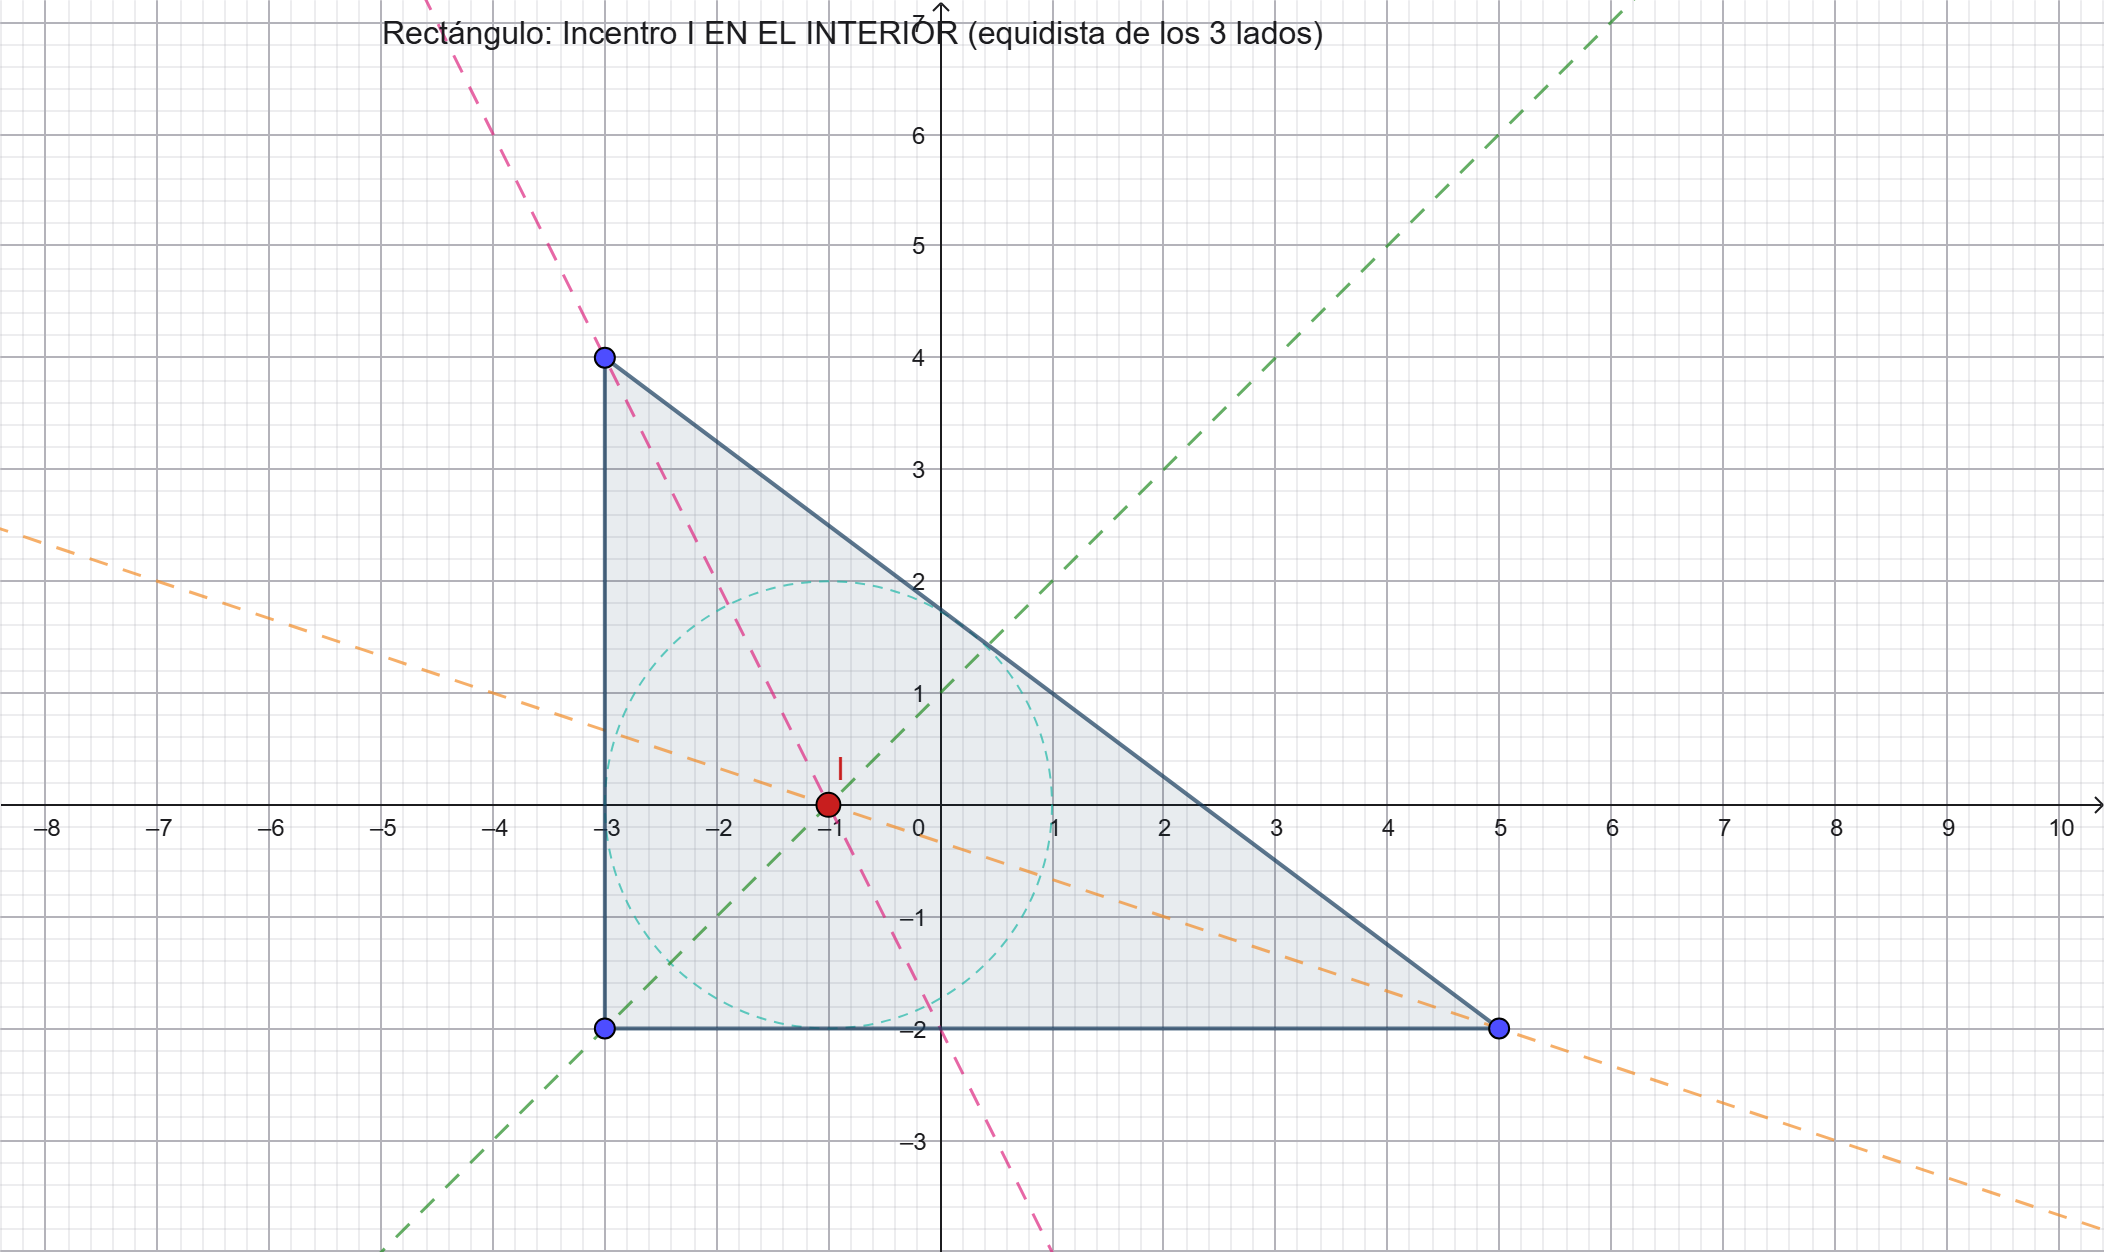
\includegraphics[width=0.32\linewidth]{img/geogebra/act2_c2_incentro_rectangulo.png}\hfill
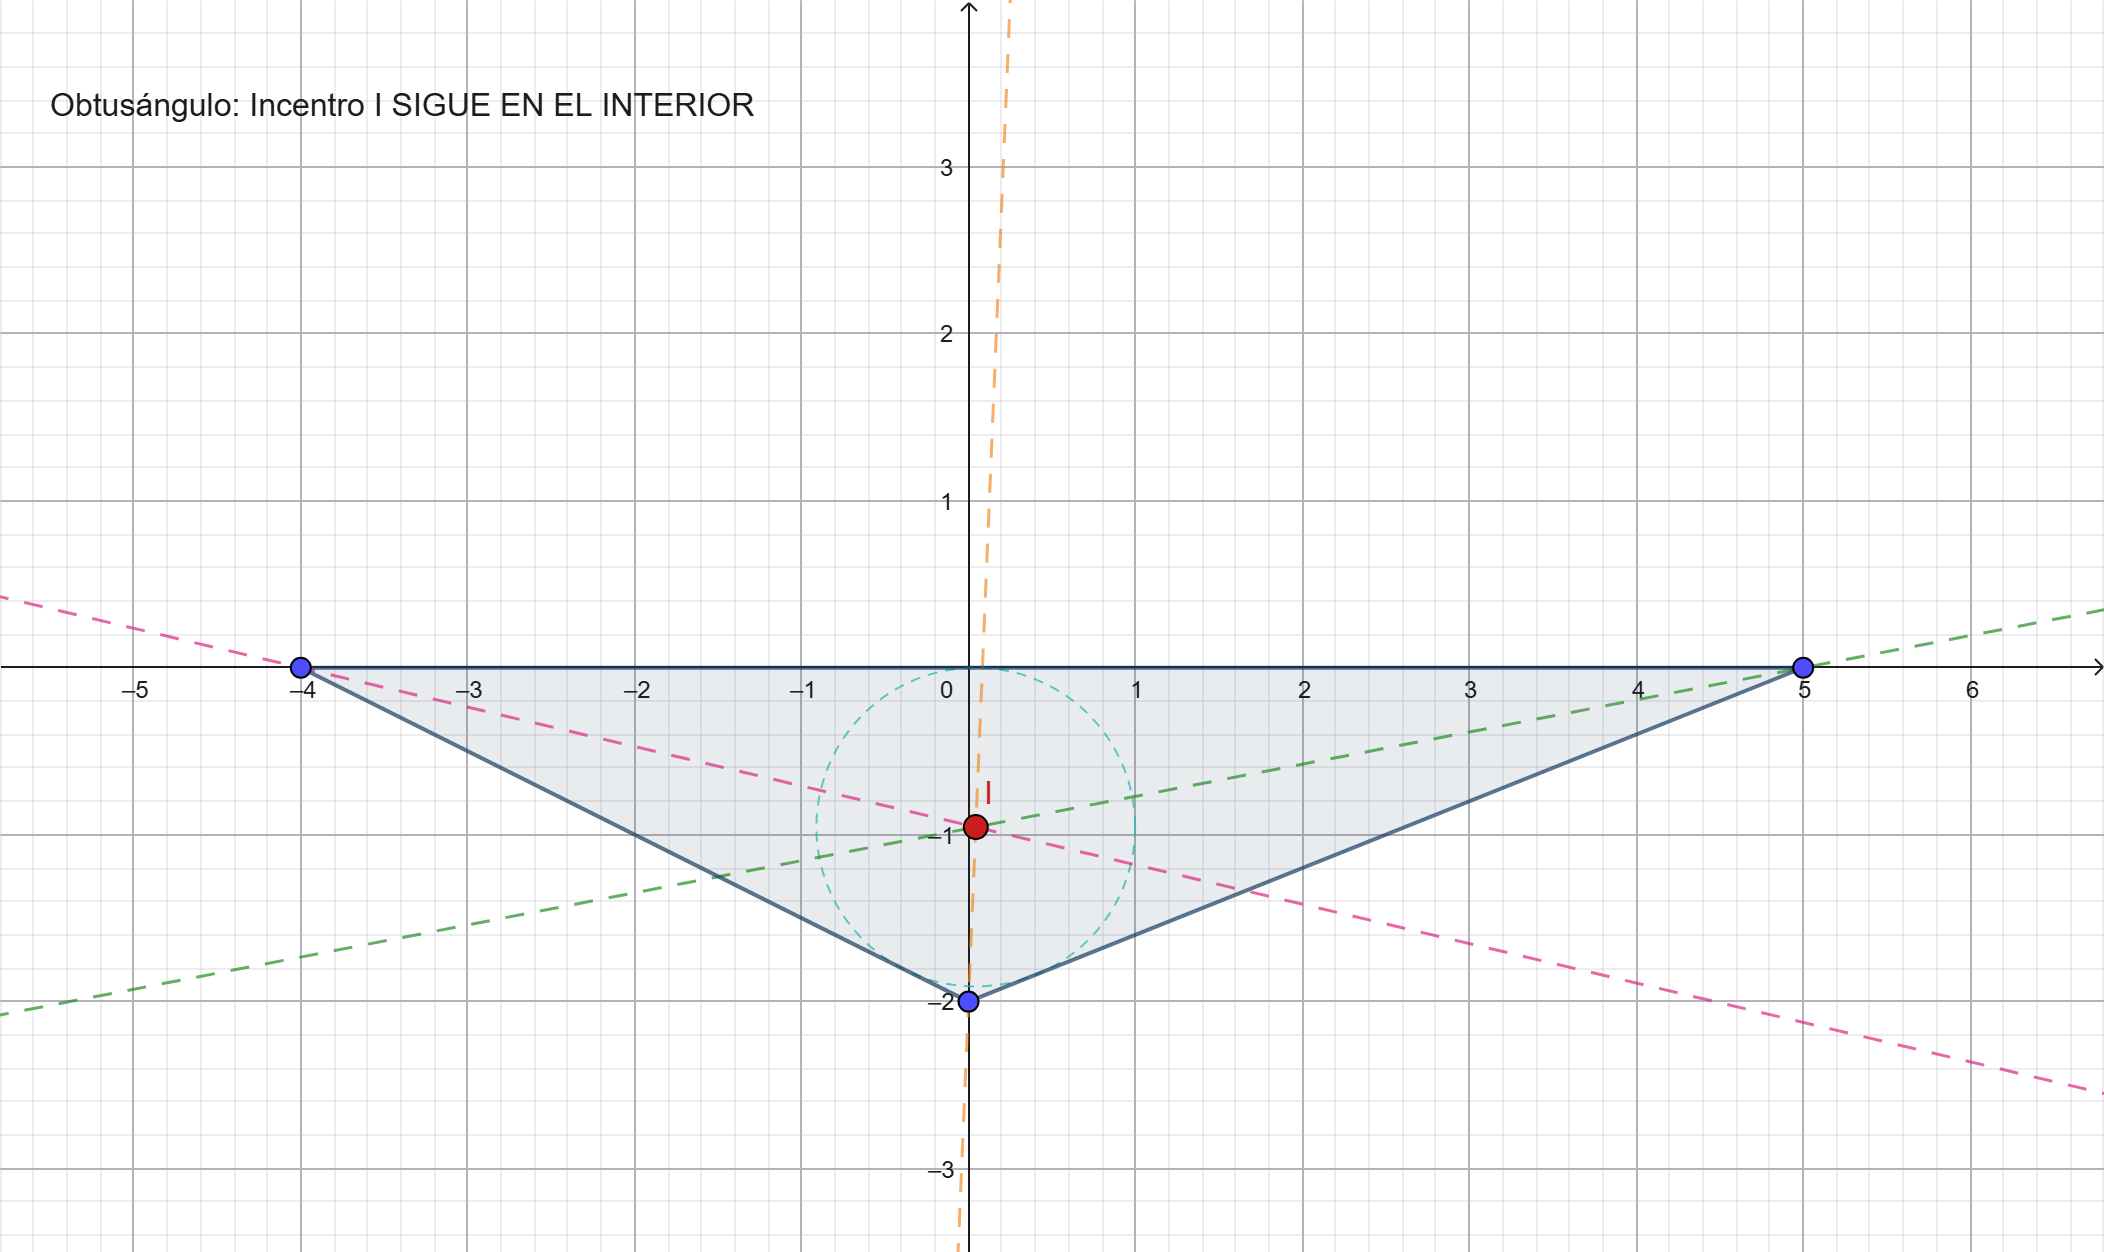
\includegraphics[width=0.32\linewidth]{img/geogebra/act2_c3_incentro_obtusangulo.png}
\caption{Actividad c (GeoGebra): Bisectrices interiores e incentro $I$ (siempre interior) en acutángulo, rectángulo y obtusángulo.}
\end{figure}

\textbf{Respuesta a la pregunta de reflexión (Actividad c):} Al modificar los vértices en cualquier forma triangular, el punto $I$ \textbf{permanece siempre en el interior del triángulo}. La característica invariante que conserva es su \textbf{equidistancia perpendicular a los tres lados} del triángulo (el radio de la circunferencia inscrita), porque cada bisectriz es el lugar geométrico de los puntos equidistantes a dos lados adyacentes.

\subsection{Actividad d. Comparación simultánea de Circuncentro $O$ e Incentro $I$}

\begin{figure}[htbp]
\centering
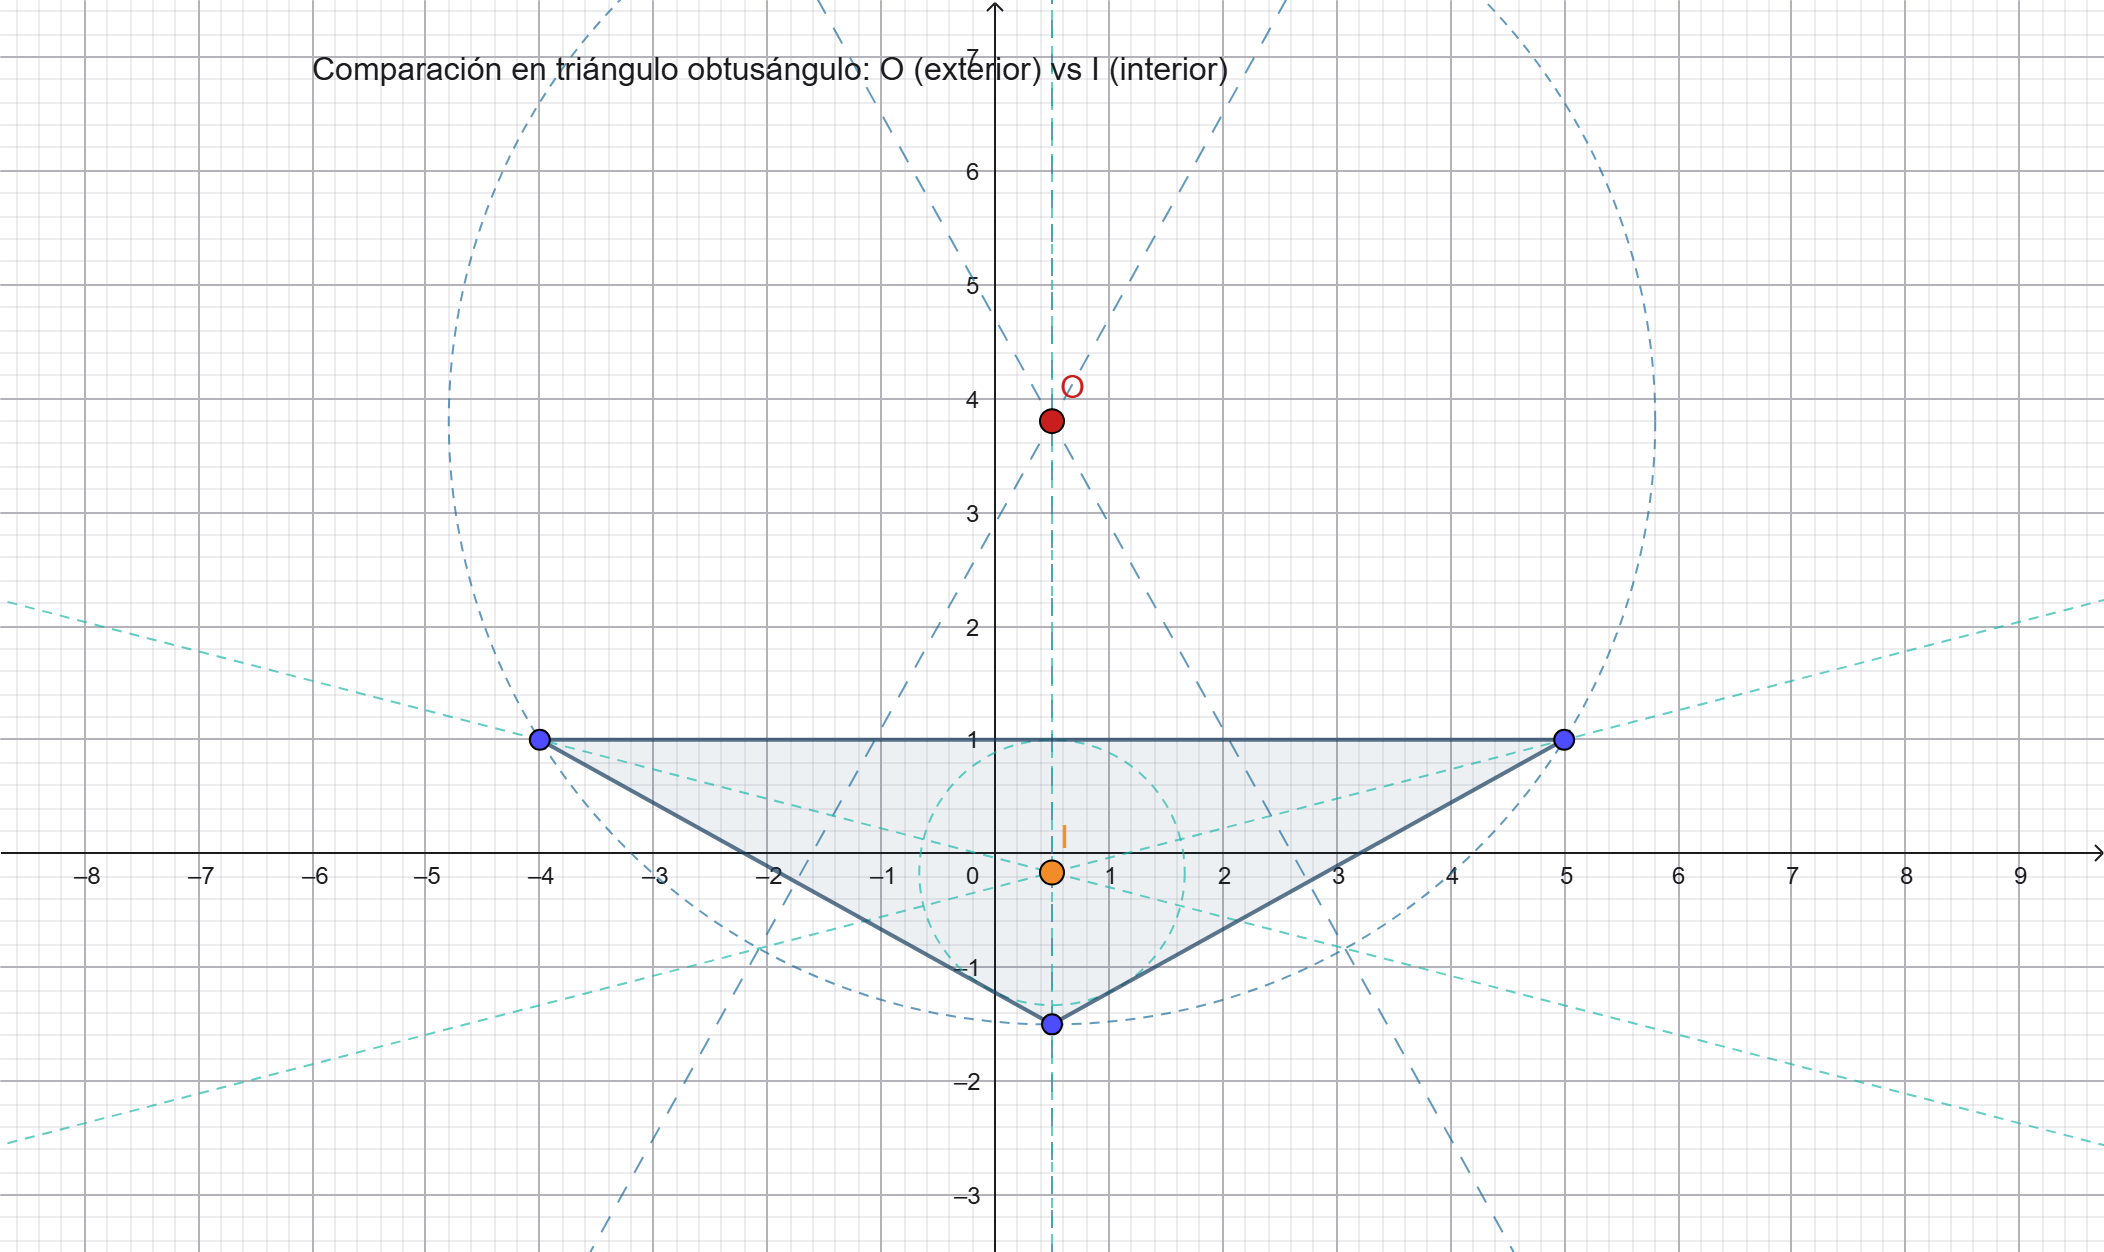
\includegraphics[width=0.80\linewidth]{img/geogebra/act2_d_comparacion_circuncentro_incentro.png}
\caption{Actividad d (GeoGebra): Contraste simultáneo de mediatrices ($O$, exterior en obtusángulo) y bisectrices ($I$, interior).}
\end{figure}

{\small\setstretch{1.1}\renewcommand{\arraystretch}{1.22}
\begin{longtable}{|>{\raggedright\arraybackslash}p{0.20\linewidth}|>{\raggedright\arraybackslash}p{0.38\linewidth}|>{\raggedright\arraybackslash}p{0.38\linewidth}|}\hline
\rowcolor{iiiepePale} \textbf{Tipo de triángulo} & \textbf{Ubicación de $O$ (Circuncentro)} & \textbf{Ubicación de $I$ (Incentro)} \\\hline
\endfirsthead\hline
\rowcolor{iiiepePale} \textbf{Tipo de triángulo} & \textbf{Ubicación de $O$ (Circuncentro)} & \textbf{Ubicación de $I$ (Incentro)} \\\hline
\endhead
Acutángulo & En el interior del triángulo. & En el interior del triángulo. \\\hline
Rectángulo & En el punto medio de la hipotenusa. & En el interior del triángulo. \\\hline
Obtusángulo & En el exterior del triángulo (opuesto al ángulo obtuso). & En el interior del triángulo. \\\hline
\end{longtable}}

\textbf{Diferencias clave entre $O$ e $I$ (Actividad d):} El circuncentro $O$ resulta de intersectar \textbf{mediatrices} de los lados (sin pasar necesariamente por los vértices), equidista de los \textbf{tres vértices} y puede ubicarse dentro, en el borde o fuera del triángulo; el incentro $I$ resulta de intersectar \textbf{bisectrices} de los ángulos interiores, equidista de los \textbf{tres lados} y siempre permanece en el interior. Solo coinciden en el triángulo equilátero.

\section{Reflexión pedagógica para el aula de secundaria}
\begin{itemize}
  \item \textbf{Dificultades al construir mediatrices y bisectrices:} Confundir mediatriz con mediana (trazar hacia el vértice opuesto en lugar de perpendicularmente), elegir una abertura del compás menor o igual a $AB/2$ impidiendo el cruce de arcos, y perder precisión en el manejo del compás sobre papel.
  \item \textbf{Ideas previas necesarias:} Concepto de distancia como menor longitud (perpendicular de punto a recta), punto medio de un segmento, ángulo y congruencia de triángulos rectángulos \citep{euclides_elementos}.
  \item \textbf{Momento de formalización:} Conviene institucionalizar los nombres \textit{circuncentro} e \textit{incentro} \textbf{después} de la fase de exploración manipulativa y dinámica en GeoGebra \citep{hohenwarter2009}, cuando los alumnos ya descubrieron la propiedad de equidistancia y necesitan nombrar un significado comprendido \citep{duval2006}.
  \item \textbf{Materiales alternativos:} Doblado de papel (papiroflexia geométrica sobre papel albanene), cuerdas tensadas en el patio, geoplanos circulares y GeoGebra clásico o en dispositivos móviles.
\end{itemize}

\clearpage
\section{Conclusiones y transferencia profesional}
La exploración conjunta de los lugares geométricos con regla, compás y GeoGebra Classic confirma nuestra tesis didáctica medular \citep{iiiepe2026_s9,hohenwarter2009}: el circuncentro $O$ y el incentro $I$ dejan de ser definiciones memorísticas cuando surgen de problemas auténticos de equidistancia respecto a vértices puntuales o a rectas concurrentes. En términos de análisis propio, se advierte que el invariante crítico radica en distinguir qué elemento permanece constante; es decir, mientras $O$ depende del ángulo máximo interior y puede emigrar fuera del triángulo en casos obtusángulos, $I$ permanece siempre interior por definición de distancia perpendicular a los tres lados \citep{duval2006}.

En consecuencia, el hallazgo pedagógico más relevante consiste en diferenciar claramente las condiciones de existencia (caso colineal degenerado frente a triángulos no degenerados) antes de introducir nomenclatura técnica. Sin embargo, para lograr una aplicación efectiva en el ejercicio profesional docente dentro de la educación secundaria \citep{sep2024_fase6}, resulta indispensable exigir demostraciones por congruencia junto al arrastre dinámico en GeoGebra, consolidando así el impacto formativo entre la percepción visual y la prueba lógica. Además, este enfoque metodológico facilita la transferencia a problemas reales de diseño espacial y localización.

Desde una perspectiva analítica propia, considero que secuenciar primero el trazo manual de arcos y posteriormente la verificación dinámica digital fortalece la comprensión estructural de la geometría euclidiana, lo cual me lleva a sostener que la tecnología educativa potencia el razonamiento únicamente cuando acompaña la argumentación deductiva en la práctica profesional.\footnote{En la elaboración de este trabajo se utilizaron herramientas de inteligencia artificial como apoyo para la organización estructural y revisión de estilo del texto, conforme a los lineamientos de integridad y ética académica institucional. El análisis conceptual, la verificación de fuentes primarias y la postura sostenida son de autoría del estudiante.}

\clearpage
\renewcommand{\refname}{Referencias}
\bibliography{referencias}

\end{document}
